\chapter{Tinjauan Pustaka dan Dasar Teori}

\section{Tinjauan Pustaka}

Penyusunan tugas akhir ini tidak terlepas dari karya-karya tulis terdahulu yang menjadi basis ataupun inspirasi penulis dalam melaksanakan seluruh rangkaian penelitian. Subbab ini berisi ulasan dan analisis karya-karya tulis tersebut serta hubungannya dengan tugas akhir ini.

Karya tulis pertama yang dibahas adalah sebuah tesis master berjudul \textit{Through the Wormhole: Cross-OS Desktop Integration for Linux Applications} yang ditulis oleh John Ingve Olsen dan dipublikasikan pada tahun 2022 \cite{olsen-2022-through-the-wormhole}. Tesis ini merupakan karya tulis yang paling signifikan dalam penyusunan tugas akhir penulis karena memiliki topik dan tujuan yang serupa dengan tugas akhir penulis dan menjadi inspirasi terbesar dalam perancangan tugas akhir penulis. Tesis ini membahas pengintegrasian sejumlah aspek antarmuka grafis Windows Subsystem for Linux (WSL) dengan \textit{host} Windows yang dicapai melalui pengembangan sejumlah perangkat lunak pembantu:
\begin{enumerate}
    \item perangkat lunak pengelola bus sesi D-Bus (\textit{session manager}) yang menyeragamkan bus perpesanan D-Bus yang dipakai oleh sesi-sesi WSL yang berbeda dan
    \item perangkat lunak "Wormhole" itu sendiri yang mengintegrasikan aspek-aspek antarmuka grafis WSL dengan \textit{desktop} Windows.
\end{enumerate}
Olsen menggunakan bahasa pemrograman Rust dalam mengembangkan kedua perangkat lunak tersebut. Aspek-aspek yang diintegrasikan dalam tesis ini yakni
\begin{itemize}
    \item ikon status (\textit{status icons}) yang umumnya muncul di sisi kanan \textit{taskbar} pada Windows,
    \item notifikasi, dan
    \item jendela dialog pemilih berkas (\textit{file chooser}).
\end{itemize}
Meskipun Wormhole merupakan satu kesatuan perangkat lunak, Wormhole terdiri dari dua buah proses yang masing-masing berjalan di sisi \textit{host} Windows (dinamakan "\textit{backend}") dan di sisi WSL (dinamakan "\textit{bridge}"). Dalam bab kelima tesis ini, Olsen menyebutkan bahwa untuk menghubungkan proses \textit{backend} Wormhole dengan proses \textit{bridge} Wormhole, terdapat tiga pilihan metode yang mungkin dilakukan: menghubungkan dengan soket TCP/IP, berkomunikasi melalui \textit{stream} standar (\textit{standard input} dan \textit{standard output}), dan menghubungkan dengan soket Hyper-V; Olsen memilih metode ketiga karena ia merasa metode tersebut tidak memiliki kelemahan bila dibandingkan dengan kedua metode lainnya meskipun pengimplementasian metode ketiga tersebut memberikan tantangan tersendiri. Satu hal yang penulis soroti dalam tesis ini yakni mekanisme penghubungan dengan bus perpesanan D-Bus; Olsen mendesain proses \textit{bridge} agar bertindak sebagai \textit{proxy} bus perpesanan D-Bus sehingga proses \textit{backend} yang terhubung dengan proses \textit{bridge} dapat mengakses bus perpesanan D-Bus tersebut layaknya secara langsung. Secara garis besar, tesis ini memiliki perbedaan dengan tugas akhir penulis dalam tiga aspek:
\begin{itemize}
    \item cakupan fungsionalitas yang diintegrasikan (tugas akhir penulis juga mengimplementasikan sistem notifikasi, serupa dengan tesis ini, tetapi dengan tambahan fungsionalitas kontrol media),
    \item metode penghubungan (\textit{bridging}) kedua lingkungan yang digunakan (tugas akhir penulis memanfaatkan metode transportasi TCP yang tersedia pada D-Bus dengan mekanisme yang cukup berbeda dengan mekanisme yang Olsen lakukan pada tesis ini), dan
    \item perlunya pengembangan perangkat lunak pengelola sesi (\textit{session manager}) D-Bus (systemd telah didukung oleh WSL sejak September 2022 \cite{systemd-support-is-now-available-in-wsl} dan telah menjadi \textit{default} pada instalasi distribusi Ubuntu di WSL sejak perilisan Ubuntu 23.04 pada April 2023 \cite{ubuntu-2304-release-roundup-systemd-now-becomes-default-for-ubuntu-on-wsl} sehingga pengelolaan sesi bus perpesanan D-Bus saat ini telah berada di bawah kontrol systemd seperti halnya pada sistem operasi Linux asli; ketiadaan pembahasan systemd dalam tesis ini mengindikasikan bahwa waktu penulisan tesis ini terjadi sebelum hadirnya dukungan systemd tersebut sehingga diperlukan pengembangan perangkat lunak \textit{session manager} tersendiri pada saat itu).
\end{itemize}

Karya tulis kedua yang dibahas adalah sebuah tesis master berjudul \textit{Notifications in a Multi-Device Environment} yang ditulis oleh Dominik Weber dan dipublikasikan pada tahun 2015 \cite{weber2015notifications}. Secara garis besar, tesis ini membahas

\section{Dasar Teori}

\subsection{Antarmuka Sistem Operasi (\textit{Shell})}

Sistem operasi tersusun atas sejumlah komponen, mulai dari komponen terdalam yang menyentuh perangkat-perangkat keras hingga komponen yang berantarmuka langsung dengan pengguna. Beberapa di antara komponen-komponen tersebut yakni \textit{kernel}, \textit{driver}, perangkat lunak sistem, \textit{shell}, dan perangkat lunak pengguna (aplikasi). Salah satu komponen yang krusial ialah \textit{shell} yang bertugas memberikan antarmuka bagi pengguna untuk dapat berinteraksi dengan sistem operasi tersebut.

Penggunaan istilah "\textit{shell}" untuk menandakan antarmuka sistem operasi pertama kali terjadi pada sekitar tahun 1964--1965 oleh Louis Pouzin ketika sedang mengembangkan sistem operasi Multics \cite{origin-of-the-shell-name}. Istilah \textit{shell} digunakan karena komponen ini adalah bagian sistem operasi terluar yang berinteraksi secara langsung dengan dunia luar dan mengelilingi komponen-komponen sistem operasi di bawahnya, sehingga dapat dianalogikan sebagai "cangkang" dari sistem operasi \cite{shell-jargon-explanation}.

Secara umum, terdapat berbagai jenis \textit{shell} yang digunakan oleh sistem-sistem operasi modern saat ini:
\begin{itemize}
    \item \textbf{\textit{Shell} berantarmuka grafis (\textit{graphical user interface})}\\
    \textit{Shell} jenis ini merupakan \textit{shell} yang paling sering pengguna temui pada zaman modern ini. Sebagian besar pengguna saat ini berinteraksi dengan perangkat komputer mereka melalui metode interaksi grafis. Antarmuka tempat pengguna berinteraksi tersebut sesungguhnya merupakan komponen \textit{shell} yang merupakan bagian dari sistem operasi pada perangkat yang bersangkutan. Sebagai contoh, \textit{shell} grafis pada sistem operasi Windows 11 terdiri atas \textit{taskbar} yang terletak di bawah layar, menu Start yang dapat dimunculkan dengan menekan tombol Start (tombol berlogo Windows di dalam \textit{taskbar}), pusat pemberitahuan/notifikasi, dan bilah pengaturan cepat (\textit{quick settings}).
    
    \item \textbf{\textit{Shell} berantarmuka baris perintah (\textit{command-line interface})}\\
    \textit{Shell} jenis ini telah ada terlebih dahulu sebelum dikembangkannya \textit{shell} berantarmuka grafis. Pada zaman modern ini, \textit{shell} berantarmuka baris perintah pun masih sering digunakan, terutama untuk kegunaan pengaksesan fungsionalitas sistem operasi tingkat lanjut, administrasi sistem, dan otomasi (\textit{scripting}). Beberapa contoh \textit{shell} berantarmuka baris perintah modern yakni PowerShell di sistem operasi Windows serta Bourne shell (\verb|sh|), Bourne-Again Shell (\verb|bash|), Z shell (\verb|zsh|), KornShell (\verb|ksh|), dan Fish shell (\verb|fish|) di sistem operasi Linux \cite{kidwai2021comparative}.
\end{itemize}

\subsection{Linux, "Mirip Unix", dan Standar POSIX}

Linux merupakan keluarga sistem operasi

\subsection{D-Bus}

D-Bus merupakan sistem komunikasi antarproses (\textit{interprocess communication}) yang populer digunakan di sebagian besar distribusi Linux. Sesuai dengan namanya, D-Bus bekerja dengan konsep arsitektur "bus" yang berarti terdapat sebuah kanal utama (bus) sebagai jalur pertukaran informasi dan terdapat sejumlah klien yang terhubung dengan kanal utama (bus) tersebut. Secara garis besar, terdapat dua komponen utama dalam penggunaan sistem D-Bus:

\begin{itemize}
    \item \textbf{\textit{Server} atau \textit{daemon} D-Bus}\\
    \textit{Server} D-Bus bertindak sebagai penyedia bus sentral tempat klien-klien D-Bus terhubung. \textit{Server} D-Bus bertugas mengelola klien-klien yang terhubung dan menyalurkan data dari sumbernya ke tujuannya dengan benar \cite{qt-introduction-to-dbus}. \textit{Server} D-Bus umumnya dijalankan oleh sebuah proses yang bernama \textit{daemon} D-Bus yang umumnya memiliki nama berkas \textit{executable} "\path{dbus-daemon}".

    \item \textbf{Klien D-Bus}\\
    Klien D-Bus merupakan istilah untuk tiap-tiap perangkat lunak yang terhubung ke bus utama D-Bus. Klien D-Bus dapat bertindak sebagai penyedia layanan (\textit{provider}) ataupun sebagai aplikasi reguler yang mengonsumsi layanan (\textit{consumer}) \textcolor{orange}{(TODO: Find the correct terminologies for those)}.
\end{itemize}

\begin{figure}
    \centering
    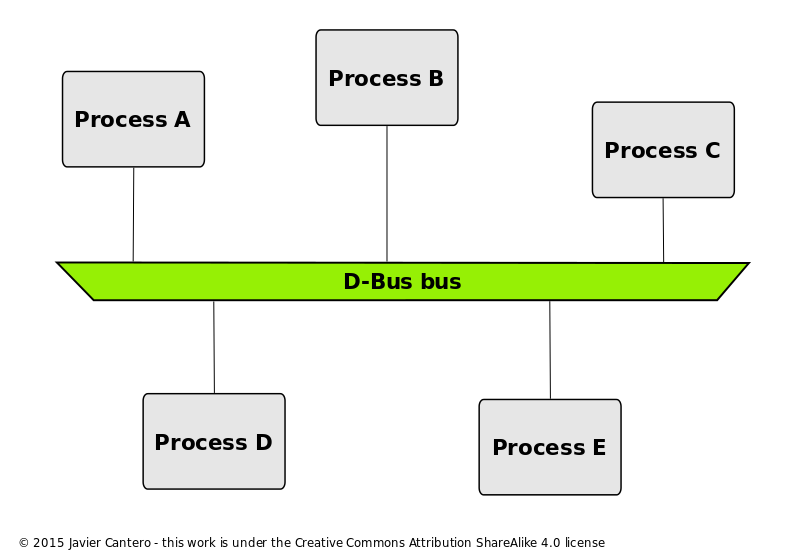
\includegraphics[width=0.75\linewidth]{archives//contents-template-pak-prapto//chapter-2/dbus-analogy-diagram.png}
    \caption{Ilustrasi bus perpesanan D-Bus \cite{dbus-bus-illustration}}
    \label{fig:enter-label}
\end{figure}

\begin{figure}
    \centering
    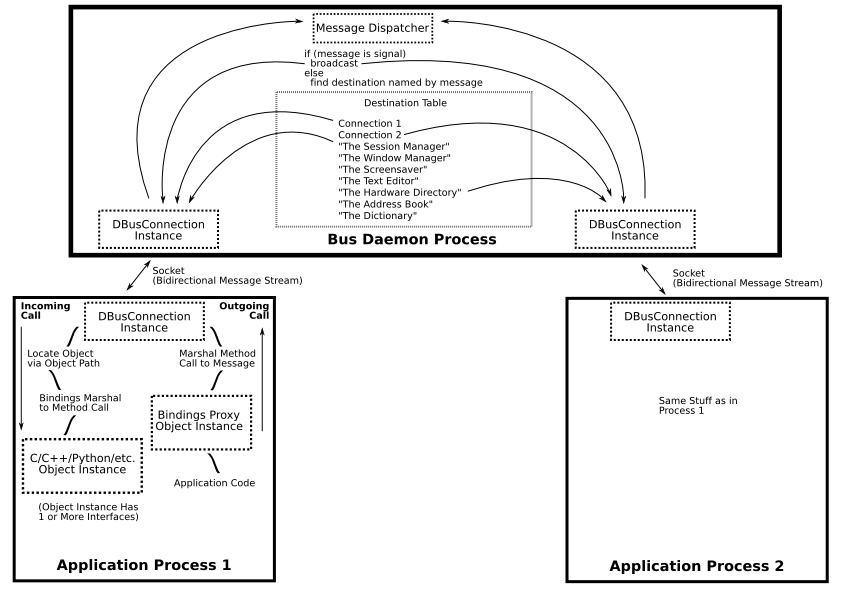
\includegraphics[width=1\linewidth]{contents//chapter-2/dbus-diagram.png}
    \caption{Diagram mendetail arsitektur D-Bus \cite{dbus-main-project-page}}
    \label{fig:enter-label}
\end{figure}

Dalam suatu sistem operasi yang sedang berjalan, dimungkinkan penjalanan lebih dari satu bus dalam satu waktu. Pada sistem operasi Linux, umumnya digunakan dua buah bus yang memiliki peran masing-masing, yaitu bus sistem (\textit{system bus}) dan bus sesi (\textit{session bus}). Bus sistem digunakan untuk mengelola dan mengadministrasi hal-hal yang bersifat penting terhadap berjalannya sistem operasi, seperti penyambungan perangkat keras baru, peringatan baterai lemah, dan status jaringan \cite{will2020trusted}. Bus sistem berjalan secara \textit{system-wide} sehingga mencakup seluruh sesi pengguna yang sedang berjalan di sistem operasi. Di sisi lain, bus sesi digunakan untuk hal-hal yang bersifat lebih mengarah ke pengguna (\textit{user-facing}) seperti pengiriman notifikasi dan sistem kontrol media, dua hal yang menjadi topik utama tugas akhir ini. Bus sesi tersedia secara lokal di tiap-tiap sesi pengguna yang sedang berjalan di suatu sistem operasi. Istilah "bus perpesanan D-Bus", "\textit{server} D-Bus", dan "\textit{daemon} D-Bus" dapat dikatakan identik dalam konteks ini; tiap-tiap bus memiliki \textit{instance} \textit{daemon} D-Bus-nya masing-masing, sehingga sistem operasi Linux secara \textit{default} memiliki dua buah \textit{instance} \textit{daemon} D-Bus yang berjalan dalam satu waktu.

Agar dapat dihubungi oleh para klien, tiap-tiap bus perpesanan D-Bus memiliki alamat yang diatur pada awal penjalanan \textit{daemon} D-Bus. Bentuk alamat yang digunakan oleh bus perpesanan D-Bus berbeda-beda sesuai dengan metode transportasi yang digunakan. Berdasarkan spesifikasi D-Bus \cite{dbus-specification}, terdapat sejumlah metode transportasi yang didukung oleh D-Bus:
\begin{itemize}
    \item \textbf{Soket Unix}\\
    Metode transportasi berbasis soket Unix menggunakan berkas soket Unix yang terletak secara lokal pada \textit{file system}. Metode transportasi ini hanya didukung apabila \textit{daemon} D-Bus berjalan di sistem operasi berbasis Unix atau mirip Unix seperti Linux dan macOS. Metode transportasi ini digunakan apabila penulisan alamat diawali oleh "\verb|unix:|".

    \item \textbf{systemd}\\
    Metode transportasi berbasis systemd memiliki konsep serupa dengan metode transportasi berbasis soket Unix, tetapi memanfaatkan sistem pengelolaan soket otomatis bernama aktivasi soket (\textit{socket activation}) yang dilakukan oleh systemd. Metode transportasi ini memanfaatkan informasi soket yang dikelola oleh systemd untuk digunakan sebagai metode transportasi D-Bus. Seperti namanya, metode transportasi ini hanya tersedia pada sistem operasi Linux yang menggunakan systemd sebagai sistem init-nya. Metode transportasi ini digunakan apabila penulisan alamat berisikan "\verb|systemd:|".
    
    \item \textbf{launchd}\\
    Metode transportasi berbasis launchd juga memiliki konsep yang serupa dengan metode transportasi berbasis soket Unix, tetapi memanfaatkan soket Unix yang telah dialokasikan oleh launchd. Mengingat sistem init launchd hanya tersedia pada sistem operasi macOS, metode transportasi ini hanya didukung apabila \textit{daemon} D-Bus berjalan di sistem operasi macOS. Metode transportasi ini digunakan apabila penulisan alamat berisikan "\verb|launchd:|".
    
    \item \textbf{TCP}\\
    Metode transportasi berbasis TCP memanfaatkan protokol TCP (Transmission Control Protocol) sebagai metode komunikasi antarklien D-Bus, baik yang terletak pada perangkat komputer yang sama maupun yang terletak pada perangkat komputer yang berbeda (\textit{remote}). Metode transportasi ini merupakan satu-satunya metode transportasi yang tersedia apabila \textit{daemon} D-Bus berjalan pada sistem operasi Windows mengingat metode-metode transportasi yang lain tidak didukung pada sistem operasi Windows. Metode transportasi ini digunakan apabila penulisan alamat diawali oleh "\verb|tcp:|" dan diikuti oleh properti-properti yang terdiri dari "\verb|host|" (wajib), "\verb|bind|" (opsional), "\verb|port|" (opsional), dan "\verb|family|" (opsional) yang penulisannya dipisahkan oleh tanda koma (misalnya "\path{tcp:localhost,port=12345,family=ipv4}").

    \item \textbf{TCP dengan metode otentikasi nonce}\\
    Metode transportasi ini identik dengan metode transportasi berbasis TCP biasa, tetapi dengan tambahan lapisan keamanan berupa otentikasi berbasis nonce. Metode otentikasi berbasis nonce memastikan bahwa hanya klien yang memiliki akses baca (\textit{read access}) pada suatu lokasi tertentu di \textit{file system} dapat terhubung ke \textit{server} D-Bus. Metode transportasi ini memiliki format penulisan alamat yang serupa dengan metode transportasi berbasis TCP biasa (sama-sama berawalan "\verb|tcp:|" dengan tambahan properti "\verb|noncefile|".

    \item \textbf{Subproses}\\
    Metode transportasi berbasis subproses bekerja dengan cara melakukan \textit{fork} pada suatu proses dan menghubungkan \textit{standard input} dan \textit{standard output} proses tersebut ke sebuah soket Unix anonim. Metode transportasi ini tidak tersedia pada sistem operasi Windows. Metode transportasi ini digunakan apabila alamat diawali oleh "\verb|unixexec:|".
\end{itemize}

Seperti yang telah disebutkan pada tiap-tiap deskripsi metode transportasi di atas, metode transportasi ditentukan secara otomatis sesuai dengan format penulisan alamat bus perpesanan D-Bus yang telah diatur. Alamat bus perpesanan D-Bus dapat diatur melalui dua tempat: argumen penjalanan \textit{daemon} D-Bus dan berkas konfigurasi. Metode pengaturan alamat bus perpesanan D-Bus melalui argumen penjalanan \textit{daemon} D-Bus dilakukan dengan menambahkan argumen berbentuk \lstinline[language=bash,columns=fixed]{--address="<tuliskan alamat yang diinginkan di sini>"}. Metode pengaturan alamat melalui argumen akan menimpa (\textit{override}) pengaturan apa pun yang dilakukan di berkas konfigurasi. Di sisi lain, metode pengaturan alamat bus perpesanan D-Bus melalui berkas konfigurasi dilakukan dengan cara memodifikasi berkas konfigurasi \textit{default} yang telah ada (berkas konfigurasi \textit{default} bus sistem berada di \path{/usr/share/dbus-1/system.conf} dan berkas konfigurasi \textit{default} bus sesi berada di \path{/usr/share/dbus-1/session.conf}) atau membuat berkas konfigurasi baru berekstensi berkas "\verb|.conf|" dan memuatnya pada saat penjalanan \textit{daemon} D-Bus melalui argumen \lstinline[language=bash,columns=fixed]{--config-file=<lokasi berkas konfigurasi>}.

Klien-klien yang terhubung dengan D-Bus mempertukarkan informasi dalam bentuk "pesan" (\textit{messages}). Tiap-tiap pesan yang dikirimkan pada D-Bus mengandung data yang dipertukarkan serta informasi pengirim dan penerima agar bisa tersampaikan ke tujuan dengan baik.

Proses interaksi di dalam D-Bus didesain agar memiliki konsep yang serupa dengan pemrograman berorientasi objek; tiap-tiap klien D-Bus dapat direpresentasikan sebagai "objek" di dalam bus perpesanan D-Bus. Meskipun demikian, klien D-Bus juga memiliki konsep-konsep yang spesifik terhadap D-Bus yang umumnya tidak ada di pemrograman berbasis objek. Berikut elemen-elemen yang dimiliki oleh klien D-Bus dalam mempertukarkan pesan.
\begin{itemize}
    \item \textbf{Sinyal (\textit{signal})}\\

    \item \textbf{Metode (\textit{method})}\\

    \item \textbf{Properti (\textit{property})}\\
\end{itemize}

Proses pertukaran informasi antarklien D-Bus dilakukan melalui elemen-elemen yang dimiliki oleh klien

Tiap-tiap klien dalam D-Bus mengemban sejumlah elemen yang berguna dalam pertukaran pesan. Berikut elemen-elemen tersebut.
\begin{itemize}
    \item Interface
\end{itemize}

Dalam pengoperasian D-Bus, terdapat sejumlah konsep perpesanan:
\begin{itemize}
    \item 
\end{itemize}

\subsection{Sistem Init systemd}

systemd merupakan salah satu sistem init yang tersedia untuk digunakan di sistem operasi Linux di samping sistem-sistem init lain seperti SysV Init, .

\subsection{Dukungan Kompatibilitas Linux atau Mirip Unix di Windows Pra-WSL}

Teknologi yang digunakan dalam skripsi ini, Windows Subsystem for Linux, bukan merupakan satu-satunya usaha yang digunakan untuk membawa kompatibilitas Linux atau Unix-like ke dalam lingkungan sistem operasi Windows. Microsoft memiliki sejarah panjang dalam membawa dukungan Linux atau mirip Unix ke dalam lingkungan Windows.

Sebelum mengembangkan WSL, Microsoft memiliki sejumlah usaha terdahulu yang bertujuan membawa dukungan Linux/Unix-like ke dalam sistem operasi Windows. Dalam proses pengembangan Windows NT yang saat ini mendasari versi-versi Windows modern (Windows 2000 dan setelahnya), Microsoft mendesain sistem operasi tersebut sedemikian rupa agar bersifat modular dan mendukung berbagai macam "subsistem". Pada awal pengembangannya, Windows NT direncanakan memiliki tiga buah subsistem, yakni subsistem Win32, subsistem OS/2 (untuk mendukung interoperabilitas dengan sistem operasi OS/2 milik IBM), dan subsistem POSIX (untuk mendukung interoperabilitas dengan sistem-sistem berbasis Linux, UNIX, atau Unix-like yang sedang populer di kalangan bisnis pada masa itu). Seiring waktu, Microsoft memutus dukungan dan pengembangan lebih lanjut terhadap subsistem OS/2 karena adanya permasalahan bisnis dengan IBM.

Berbeda dengan subsistem OS/2 yang telah mati, dukungan dan pengembangan terhadap subsistem POSIX masih terus berjalan. Secara umum, terdapat tiga iterasi teknologi subsistem POSIX/UNIX yang dikembangkan oleh Microsoft:

\begin{enumerate}
    \item \textbf{Microsoft POSIX Subsystem.} Teknologi ini merupakan teknologi asli kembangan Microsoft yang ada sejak awal pengembangan Windows NT. Teknologi ini tersedia untuk sistem operasi Windows NT 3.1 hingga Windows 2000.
    \item \textbf{Windows Services for Unix (SFU).} Produk ini sesungguhnya adalah teknologi milik perusahaan bernama PTS yang dilisensikan kepada Microsoft. Produk ini menggantikan Microsoft POSIX Subsystem sejak sistem operasi Windows XP dan Windows Server 2003.
    %Teknologi yang membawahi (...) ini sejatinya merupakan hasil pengembangan
    \item \textbf{Subsystem for Unix-based Applications (SUA).}
    % Teknologi ini sejatinya merupakan pengembangan lebih lanjut dari SFU.
    % Teknologi ini pada awalnya bernama subsistem Interix dan berganti nama setelah Microsoft mengakuisisi perusahaan pengembangnya. Setelah akuisisi, produk ini tidak lagi berdiri sebagai produk terpisah, tetapi menjadi salah satu komponen dari Windows Services for Unix (SFU). Komponen ini tersedia sejak 
\end{enumerate}

% Reason against elaborationg further: The lack of new sources due to the nature of this topic that is "historical information".

% https://link.springer.com/chapter/10.1007/978-1-4842-6038-8_1

Di samping solusi-solusi yang [telah] ditawarkan oleh Microsoft tersebut, terdapat pula beragam solusi-solusi pihak ketiga yang meraih tujuan yang sama. Solusi-solusi pihak ketiga ini ada baik guna mengisi kekosongan dukungan oleh Microsoft secara langsung maupun sebagai substitusi (\textit{substitute}) yang menggantikan solusi bawaan milik/buatan Microsoft karena [mungkin] solusi tersebut dirasa kurang atau masih belum sempurna.

\begin{enumerate}
    \item \textbf{Colinux.}

    \item \textbf{Cygwin.}
\end{enumerate}

\subsection{Windows Subsystem for Linux (WSL)}

Windows Subsystem for Linux merupakan usaha terbaru Microsoft dalam membawa kompatibilitas Unix/Linux ke dalam lingkungan Windows.

\subsection{Dukungan Kompatibilitas Linux atau \textit{Unix-like} di Windows oleh Pihak Ketiga}

Microsoft tidak sendirian dalam mengembangkan dukungan lingkungan Linux atau \textit{Unix-like} ke dalam sistem operasi Windows; terdapat beragam pilihan pihak ketiga yang dapat membawa dukungan lingkungan Linux atau \textit{Unix-like} ke Windows.

\subsection{Teknologi Sistem Perjendelaan (\textit{Windowing System}) Linux: X11/Xorg dan Wayland}

\subsection{Windows Subsystem for Linux GUI (WSLg)}

Microsoft pertama kali menyatakan dukungan penjalanan perangkat lunak berantarmuka grafis (GUI) di Windows Subsystem for Linux versi 2 (WSL2) secara bawaan (\textit{built-in}) pada perhelatan pengembang tahunan Microsoft Build 2021.

Dalam pengembangan fungsionalitas antarmuka grafis pada Windows Subsystem for Linux, Microsoft berkomitmen untuk mengikuti standar yang telah ada pada lingkungan Linux.

\begin{figure}
    \centering
    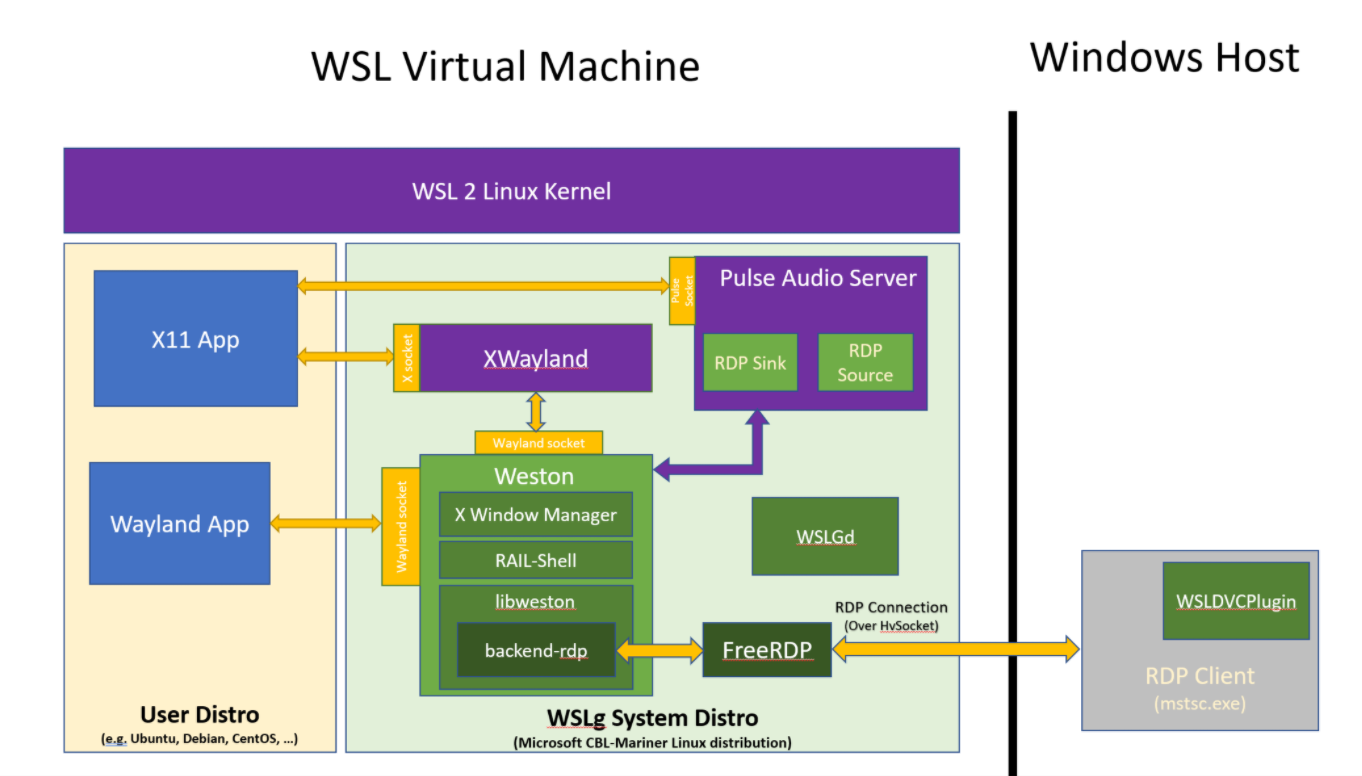
\includegraphics[width=0.5\linewidth]{wslg-architecture.png}
    \caption{Arsitektur Windows Subsystem for Linux GUI (WSLg)}
    \label{fig:enter-label}
\end{figure}

% https://link.springer.com/chapter/10.1007/978-1-4842-6873-5_1
% https://devblogs.microsoft.com/commandline/wslg-architecture/


\subsection{\textit{Media Player Remote Interfacing Specification} (MPRIS)}

\subsection{Windows API: System Media Transport Controls (SMTC)}

\subsection{\textit{Standard Stream}, Mekanisme \textit{Piping}, dan Soket}

\section{Analisis Perbandingan Metode}

Pengerjaan serta pencapaian tujuan skripsi ini, terutama mengenai penghubungan (\textit{bridging}) lingkungan Windows Subsystem for Linux (WSL) dengan lingkungan \textit{host} Windows, dapat ditempuh melalui berbagai macam metode. Setelah meninjau berbagai macam pustaka yang telah ada serta melakukan riset tentang teknologi terkait, penulis merumuskan enam macam pendekatan yang mungkin dilakukan:
\begin{enumerate}
    \item Lingkungan WSL dihubungkan dengan lingkungan \textit{host} Windows melalui \textit{socket} Unix. Hal ini dimungkinkan dengan diperkenalkannya dukungan \textit{socket} Unix (AF\_UNIX) pada sistem operasi Windows 10 ke atas pada tahun 2017 \cite{bringing-afunix-to-windows}. Penelusuran lebih lanjut mengindikasikan bahwa kemampuan ini rupanya hanya mendukung Windows Subsystem for Linux versi 1 (WSL1) dan belum mendukung Windows Subsystem for Linux versi 2 (WSL2) \cite{github-issues-afunix-not-supported-in-wsl2}. Oleh karena itu, mengingat kemampuan grafis (\textit{graphical user interface}) pada Windows Subsystem for Linux hanya tersedia pada Windows Subsytem for Linux versi 2 (WSL2), metode ini tidak relevan dengan tujuan skripsi ini.
    
    \item Lingkungan WSL dihubungkan dengan lingkungan \textit{host} Windows dengan memanfaatkan \textit{server} HTTP. Metode ini ikut dipertimbangkan mengingat pengalaman penulis yang cukup banyak berhubungan dengan bidang pengembangan web (\textit{web development}). Metode ini dapat dibagi kembali menjadi dua submetode:
    
    \begin{enumerate}
        \item Penghubungan kedua lingkungan melibatkan dua buah \textit{server} HTTP yang masing-masing berjalan di sisi WSL dan di sisi \textit{host} Windows. Dua buah \textit{server} diperlukan karena komunikasi bersifat dua arah: WSL mengirimkan konten yang ingin ditampilkan ke sisi \textit{host} Windows dan \textit{host} Windows mengomunikasikan hasil interaksi pengguna (\textit{user input}) kembali ke sisi WSL. Meskipun implementasi submetode ini dapat dibuat seefisien mungkin, penjalanan dua buah \textit{server} tetap saja terasa kurang efisien, terutama bila dibandingkan dengan metode-metode lainnya.
        
        \item Penghubungan kedua lingkungan menggunakan cukup satu buah \textit{server} saja untuk menghindari duplikasi penggunaan \textit{resources}, tetapi memanfaatkan teknologi yang memungkinkan komunikasi secara dua arah seperti HTTP \textit{long polling} dan WebSocket. Penggunaan HTTP \textit{long polling} memiliki kemungkinan menghasilkan performa yang kurang efisien \cite{problems-in-http-long-polling}, sedangkan penggunaan WebSocket sama saja dengan penggunaan Unix \textit{socket} biasa namun dengan \textit{overhead} protokol HTTP yang dapat berefek pada performa.
    \end{enumerate}
    
    \item Lingkungan WSL dihubungkan dengan lingkungan \textit{host} Windows dengan komunikasi secara tekstual atau terserialisasi (\textit{serialized}). Pertukaran informasi berbentuk teks (tekstual) ini dapat melalui berbagai perantara; berikut beberapa di antaranya.
    \begin{enumerate}
        \item Informasi tekstual dipertukarkan melalui berkas \textit{executable} pembantu (\textit{helper}) sebagai argumen pengeksekusian berkas \textit{executable} tersebut. Ditentukan dua buah berkas \textit{executable} yang masing-masing bertugas mengirimkan informasi ke sisi \textit{host} Windows dan mengirimkan informasi ke sisi WSL. Pada sisi WSL, hal ini dimungkinkan oleh kemampuan WSL menjalankan berkas \textit{executable} Windows (umumnya berekstensi \verb|.exe|) secara langsung di dalam \textit{command-line} WSL \cite{msdocs-run-windows-tools-from-linux}. Pada sisi Windows, hal ini dimungkinkan oleh kemampuan memanggil WSL secara programatik atau \textit{scripted} dengan perintah yang telah ditetapkan. Sebagai contoh, pengiriman informasi dari sisi WSL dapat dilakukan dengan perintah
        \begin{lstlisting}[language=bash]
# Di shell bash
/path/to/fwsl-send-to-windows.exe --data="<insert JSON-serialized data here>"\end{lstlisting}
        dan pengiriman informasi dari sisi Windows ke sisi WSL dapat dilakukan dengan perintah
        \begin{lstlisting}
# Di shell PowerShell atau cmd.exe
wsl.exe /path/to/fwsl-send-to-wsl --data="<insert JSON-serialized data here>"\end{lstlisting}

        \item Informasi tekstual dipertukarkan melalui mekanisme \textit{piping}. Cara pertukaran data ini serupa dengan penggunaan berkas \textit{executable} pembantu (\textit{helper}) pada submetode (a), namun data disalurkan melalui \textit{standard stream} (seperti \textit{standard input} dan \textit{standard output}) dan dihubungkan dengan \textit{pipe} alih-alih diletakkan sebagai argumen suatu berkas \textit{executable}. Pertukaran data dengan cara ini tetap memerlukan berkas-berkas \textit{executable} sebagai pengirim dan/atau penerima data. Tetapi, berbeda dengan submetode (a), submetode ini memungkinkan penggunaan perangkat lunak utama itu sendiri sebagai pengirim dan penerima data \textcolor{orange}{(TODO: Elaborate more about the programs)}. Pertukaran data difasilitasi oleh berkas \textit{named pipe} sebanyak dua buah yang masing-masing menangani pengiriman data ke tiap-tiap arah (menuju Windows dan menuju WSL).
        \begin{verbatim}
 ________________               ________________
|                |             |                |
|           StdIn(== ← === ← ==(StdOut          |
|    Windows     |             |   WSL bridge   |
|    bridge      |             |                |
|          StdOut)== → === → ==)StdIn           |
|________________|             |________________|

        \end{verbatim}

        \item Informasi tekstual dipertukarkan dengan memanfaatkan perintah \verb|dbus-send| dan \verb|dbus-monitor| secara programatik. Mengingat topik utama skripsi ini selalu berkaitan dengan protokol D-Bus, submetode ini dapat mensimplifikasi rangkaian proses pengerjaan karena menggunakan peralatan yang berasal dari D-Bus itu sendiri. Sebagai contoh, dengan pemantauan keluaran (\textit{output}) perintah \verb|dbus-monitor|, pemulaian pemutaran media (musik, video, dan lain-lain) dari suatu perangkat lunak yang berjalan di dalam WSL menghasilkan keluaran
        \begin{lstlisting}
signal time=1702386858.242218 sender=:1.19 -> destination=(null destination) serial=24 path=/org/mpris/MediaPlayer2; interface=org.freedesktop.DBus.Properties; member=PropertiesChanged
   string "org.mpris.MediaPlayer2.Player"
   array [
      dict entry(
         string "PlaybackStatus"
         variant             string "Playing"
      )
   ]
   array [
   ]\end{lstlisting}
        dan apabila pemutaran media tersebut ingin dijeda (\textit{pause}), dapat dijalankan perintah berikut
        \begin{lstlisting}[language=bash]
            dbus-send (TODO: FIND THE EXACT COMMAND)\end{lstlisting}
        Meskipun demikian, proses integrasi dalam skripsi ini melibatkan lebih dari sekadar perintah-perintah D-Bus dan dapat dipastikan membutuhkan perangkat lunak tambahan, sehingga akan lebih baik apabila seluruh fungsionalitas dan logika dalam pengerjaan skripsi ini disatukan ke dalam perangkat lunak tambahan tersebut. Selain itu, keluaran (\textit{output}) perintah \verb|dbus-monitor| tidak selalu lengkap (pada contoh keluaran perintah \verb|dbus-monitor| di atas, tidak ada informasi bahwa perangkat lunak Spotify adalah perangkat lunak yang memulai memainkan media), sehingga submetode ini kurang bisa diandalkan.
    \end{enumerate}
    
    \item Lingkungan Windows Subsystem for Linux (WSL) dihubungkan dengan lingkungan \textit{host} Windows dengan meng-\textit{extend} jangkauan bus perpesanan D-Bus hingga dapat diakses secara langsung di dalam lingkungan Windows. Hal ini dicapai dengan cara mengatur konfigurasi \verb|dbus-daemon| di WSL agar dapat diakses melalui TCP (di samping konfigurasi soket Unix \textit{default} yang telah ada) dan mengonsumsi alamat TCP yang ditentukan di perangkat lunak \textit{bridge} yang berjalan di Windows. Metode ini memiliki keuntungan tersendiri: mengingat koneksi bus perpesanan D-Bus saat ini tersedia secara langsung di lingkungan Windows, penyediaan \textit{notification server} dan \textit{MPRIS server} dapat dilakukan secara langsung oleh perangkat lunak \textit{bridge} di sisi Windows, sehingga menghilangkan kebutuhan penjalanan perangkat lunak \textit{bridge} kedua di lingkungan WSL.
        
\end{enumerate}

Setelah melalui berbagai pertimbangan di atas, metode keenam dirasa paling cocok diterapkan dalam pengerjaan skripsi ini.

\section{Pertanyaan Tugas Akhir}

Dalam serangkaian pengerjaan tugas akhir ini, penulis menemukan beberapa pertanyaan yang berkaitan dengan metode yang telah dipilih. Pertanyaan-pertanyaan ini perlu dijawab sebelum dapat melanjutkan ke langkah selanjutnya dalam pengerjaan.

\begin{enumerate}
    \item Perangkat lunak \verb|dbus-daemon| dapat melakukan \textit{listening} ke lebih dari satu alamat apabila telah diatur pada berkas konfigurasi (misalnya pada berkas \path{/usr/share/dbus-1/session.conf} untuk bus \textit{session}). Namun, \verb|dbus-daemon| juga memiliki seperangkat argumen eksekusi \cite{dbus-daemon-man-page} yang beberapa di antaranya dapat menimpa (\textit{override}) konfigurasi yang telah dilakukan pada berkas konfigurasi; salah satu argumen yang menarik perhatian yaitu argumen \verb|--address|. Apakah argumen ini mendukung pemberian lebih dari satu alamat? Apabila argumen ini hanya mendukung satu alamat, apa yang terjadi jika argumen ini digunakan dalam pemanggilan \verb|dbus-daemon| saat konfigurasi yang tertimpa (\textit{override}) pada berkas konfigurasi memuat lebih dari satu alamat? Apakah penggunaan argumen ini hanya menimpa (\textit{override}) satu buah alamat pada berkas konfigurasi saja atau menimpa (\textit{override}) semua alamat yang telah diatur pada berkas konfigurasi?

    \item Selain berkomunikasi secara lokal melalui \textit{socket} Unix, D-Bus juga memiliki kemampuan melalui protokol TCP, sehingga memungkinkan komunikasi dengan klien-klien yang berjalan di lingkungan di luar sistem operasi saat ini, baik di perangkat komputer lain (penghubungan secara \textit{remote}) maupun di sebuah \textit{virtual machine} pada perangkat komputer fisik yang sama. Apakah komputer lain tersebut memerlukan penjalanan \verb|dbus-daemon| milik komputer itu sendiri atau perangkat lunak \textit{client} di komputer tersebut dapat langsung terhubung ke D-Bus pusat tanpa memerlukan adanya \verb|dbus-daemon| tambahan yang berjalan pada komputer tersebut? (TODO: Rephrase this one.)
\end{enumerate}
